\documentclass[../ThesisDoc]{subfiles}
\begin{document}

\providecommand{\rootdir}{..}
\providecommand{\seccmd}[1]{\section{#1}}


Class coherence enforces institution restrictions (and common sense).
Coherence value is completely independent of who's assessed it.
Because of the latter, this kind coherence isn't assessed at contexts
in the implementation, but rather immediately after class/candidate creation.

% % % % % % % % % % % % % % % % % % % % % % % % % % % % % % % % % % % % % % % %
\seccmd{Capabilities}

Represent \emph{strong} restrictions, set by the institution.
Setting \emph{mode} has no effect on evaluation.

All the relations should yield either \emph{true} or \emph{false}.
A candidate is declared coherent if all the relations are \emph{true}.

Following \emph{binary} relations are defined over \emph{class data}:
\begin{itemize}
  \item \emph{group} wants to take classes of \emph{discipline};
  \item \emph{professor} can teach \emph{discipline};
  \item \emph{classroom} is equipped for \emph{discipline};
  \item \emph{classroom} has enough seats for whole \emph{group}.
\end{itemize}

Single \emph{whole-graph} relation is defined over whole candidate (set of classes):
each group must have the exact classes duration, defined by the disciplines chosen.

An agent should be keeping the capabilities of known agents, to avoid creation
of unacceptable classes.

\begin{figure}[h]
  \centering
  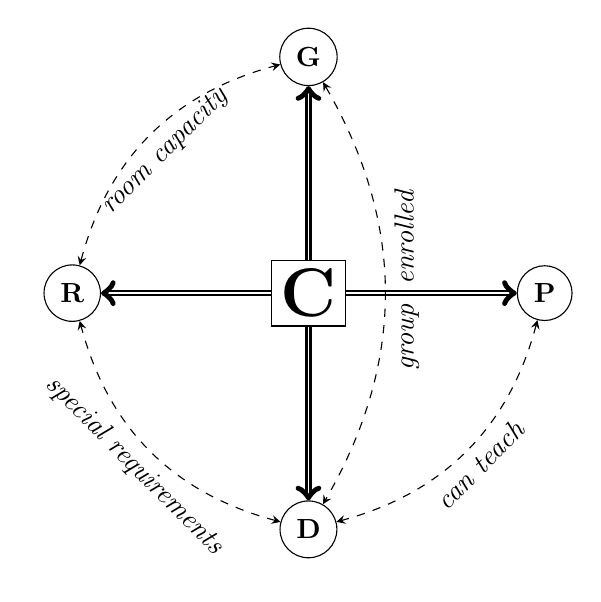
\begin{tikzpicture}

\edef\r{3cm}

\node[draw]         (C) at (0,  0) {\textbf{\Huge C}};
\node[draw, circle] (G) at (0, \r) {\textbf{G}};
\node[draw, circle] (P) at (\r, 0) {\textbf{P}};
\node[draw, circle] (D) at (0,-\r) {\textbf{D}};
\node[draw, circle] (R) at (-\r,0) {\textbf{R}};

\foreach \i in {(G),(P),(D),(R)}
 \draw[->, thick, double] (C) -- \i;

\def\data{ P/D/can teach
         , D/R/special requirements
         , R/G/room capacity
         , G/D/\quad group~~enrolled
         }

\foreach \i/\j/\k in \data
 \draw[<->, >=stealth, dashed] (\i) to[bend left
                                      ,edge node={node [sloped, below] {\emph{\k}}}]
                               (\j);


\end{tikzpicture}

  \caption{Capabilities required to form a \emph{class}.}
  \label{fig:capabilities}
\end{figure}


% % % % % % % % % % % % % % % % % % % % % % % % % % % % % % % % % % % % % % % %
\seccmd{Time Consistency}

Asserts that all the classes are consistent in time (do not intersect).

Defines a single \emph{binary} relation over classes.
Two classes are \emph{incoherent} when:
\begin{enumerate}
  \item both classes reference same group, professor or/and classroom;
  \item both classes are on the same day and their time intersect:
          either the beginning or end time of one class is in between of
          beginning and end time of another.
\end{enumerate}

\begin{center}
  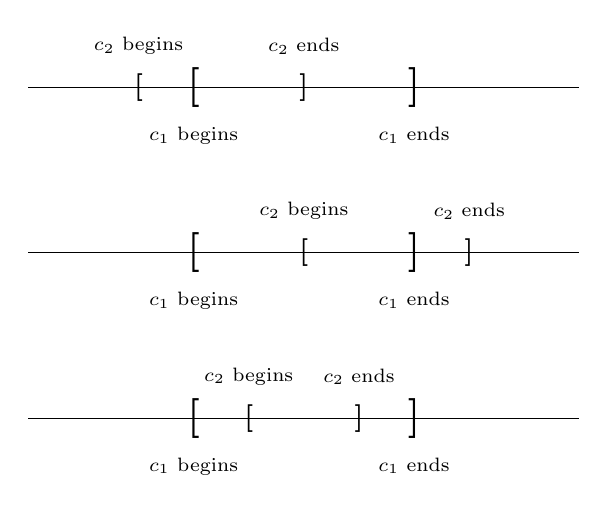
\begin{tikzpicture}[scale=0.7]

\newcommand{\plotTimeI}[3]{
  \node [label=above:{\scriptsize #3 begins}] at (#1,0) {\textbf{[}};
  \node [label=above:{\scriptsize #3 ends}]   at (#2,0) {\textbf{]}};
}

\newcommand{\plotTimeIL}[3]{
  \node [label=below:{\scriptsize #3 begins}] at (#1,0) {\textbf{\Large [}};
  \node [label=below:{\scriptsize #3 ends}]   at (#2,0) {\textbf{\Large ]}};
}


\newcommand{\plotTimeA}{
    \draw (0,0) -- (10,0);
    \plotTimeIL{3}{7}{$c_1$}
}

\begin{scope}
  \plotTimeA
  \plotTimeI{2}{5}{$c_2$}
\end{scope}

\begin{scope} [shift={(0,-3)}]
  \plotTimeA
  \plotTimeI{5}{8}{$c_2$}
\end{scope}

\begin{scope} [shift={(0,-6)}]
  \plotTimeA
  \plotTimeI{4}{6}{$c_2$}
\end{scope}

\end{tikzpicture}

\end{center}


\end{document}
